In this section, we want to motivate the advantage of the numerical smoothing idea in the context of MLMC method. For this aim we consider two examples: i) the first one is for computing the price of a digital option (see Section \ref{sec: MLMC for digital options}) , and ii) the second example is for approximating a density function with application to computing Greeks of options having non smooth payoff (see Section \ref{sec: MLMC for approximating densities and greeks}). The results  of the first example can be generalized for any kind of option having low regularity in the payoff function. On the other hand, the second example have two important applications: i) computing density functions which involves the use of Dirac functions and which is hard to approximate its expectation using MLMC due to the infinite variance, and ii) computing Greeks for an option with a non smooth payoff function.


\subsection{MLMC for digital options}\label{sec: MLMC for digital options}
In this section, we motivate the idea of using the numerical smoothing idea to compute option prices for non smooth payoff function. As an illustration, we choose the digital option as an example with parameters: $S_0=K=100$, $T=1$, $r= 0$, and   $\sigma=0.2$, and we compare MLMC results with the original payoff function (without numerical smoothing), given by Figure \ref{fig:euler_digital_without_smoothing},  and MLMC results after applying our numerical smoothing idea, given by Figure \ref{fig:euler_digital_with_smoothing}. From these two Figures we have the following conclusions:
\begin{enumerate}
\item The numerical smoothing has improved the rate of strong convergence from $1/2$ (without smoothing) to $1$ after doing the numerical smoothing (compare both top left plots in Figures \ref{fig:euler_digital_without_smoothing} and Figure \ref{fig:euler_digital_with_smoothing}.
\item The numerical smoothing has also dropped significantly the kurtosis by a factor $100$, this is can be seen clearly by comparing the middle right plots in both Figures \ref{fig:euler_digital_without_smoothing} and Figure \ref{fig:euler_digital_with_smoothing}.
\item Finally, improving the strong error rate after using the numerical smoothing, resulted in an improvement of the complexity rate going from $TOL^{-2.5}$ for the case without smoothing to  $TOL^{-2} \abs{\log TOL}^2$ for the case where MLMC is coupled with numerical smoothing (compare the bottom right plots in Figures \ref{fig:euler_digital_without_smoothing} and \ref{fig:euler_digital_with_smoothing}).
\end{enumerate}

\FloatBarrier
	\begin{figure}[h!]
\centering
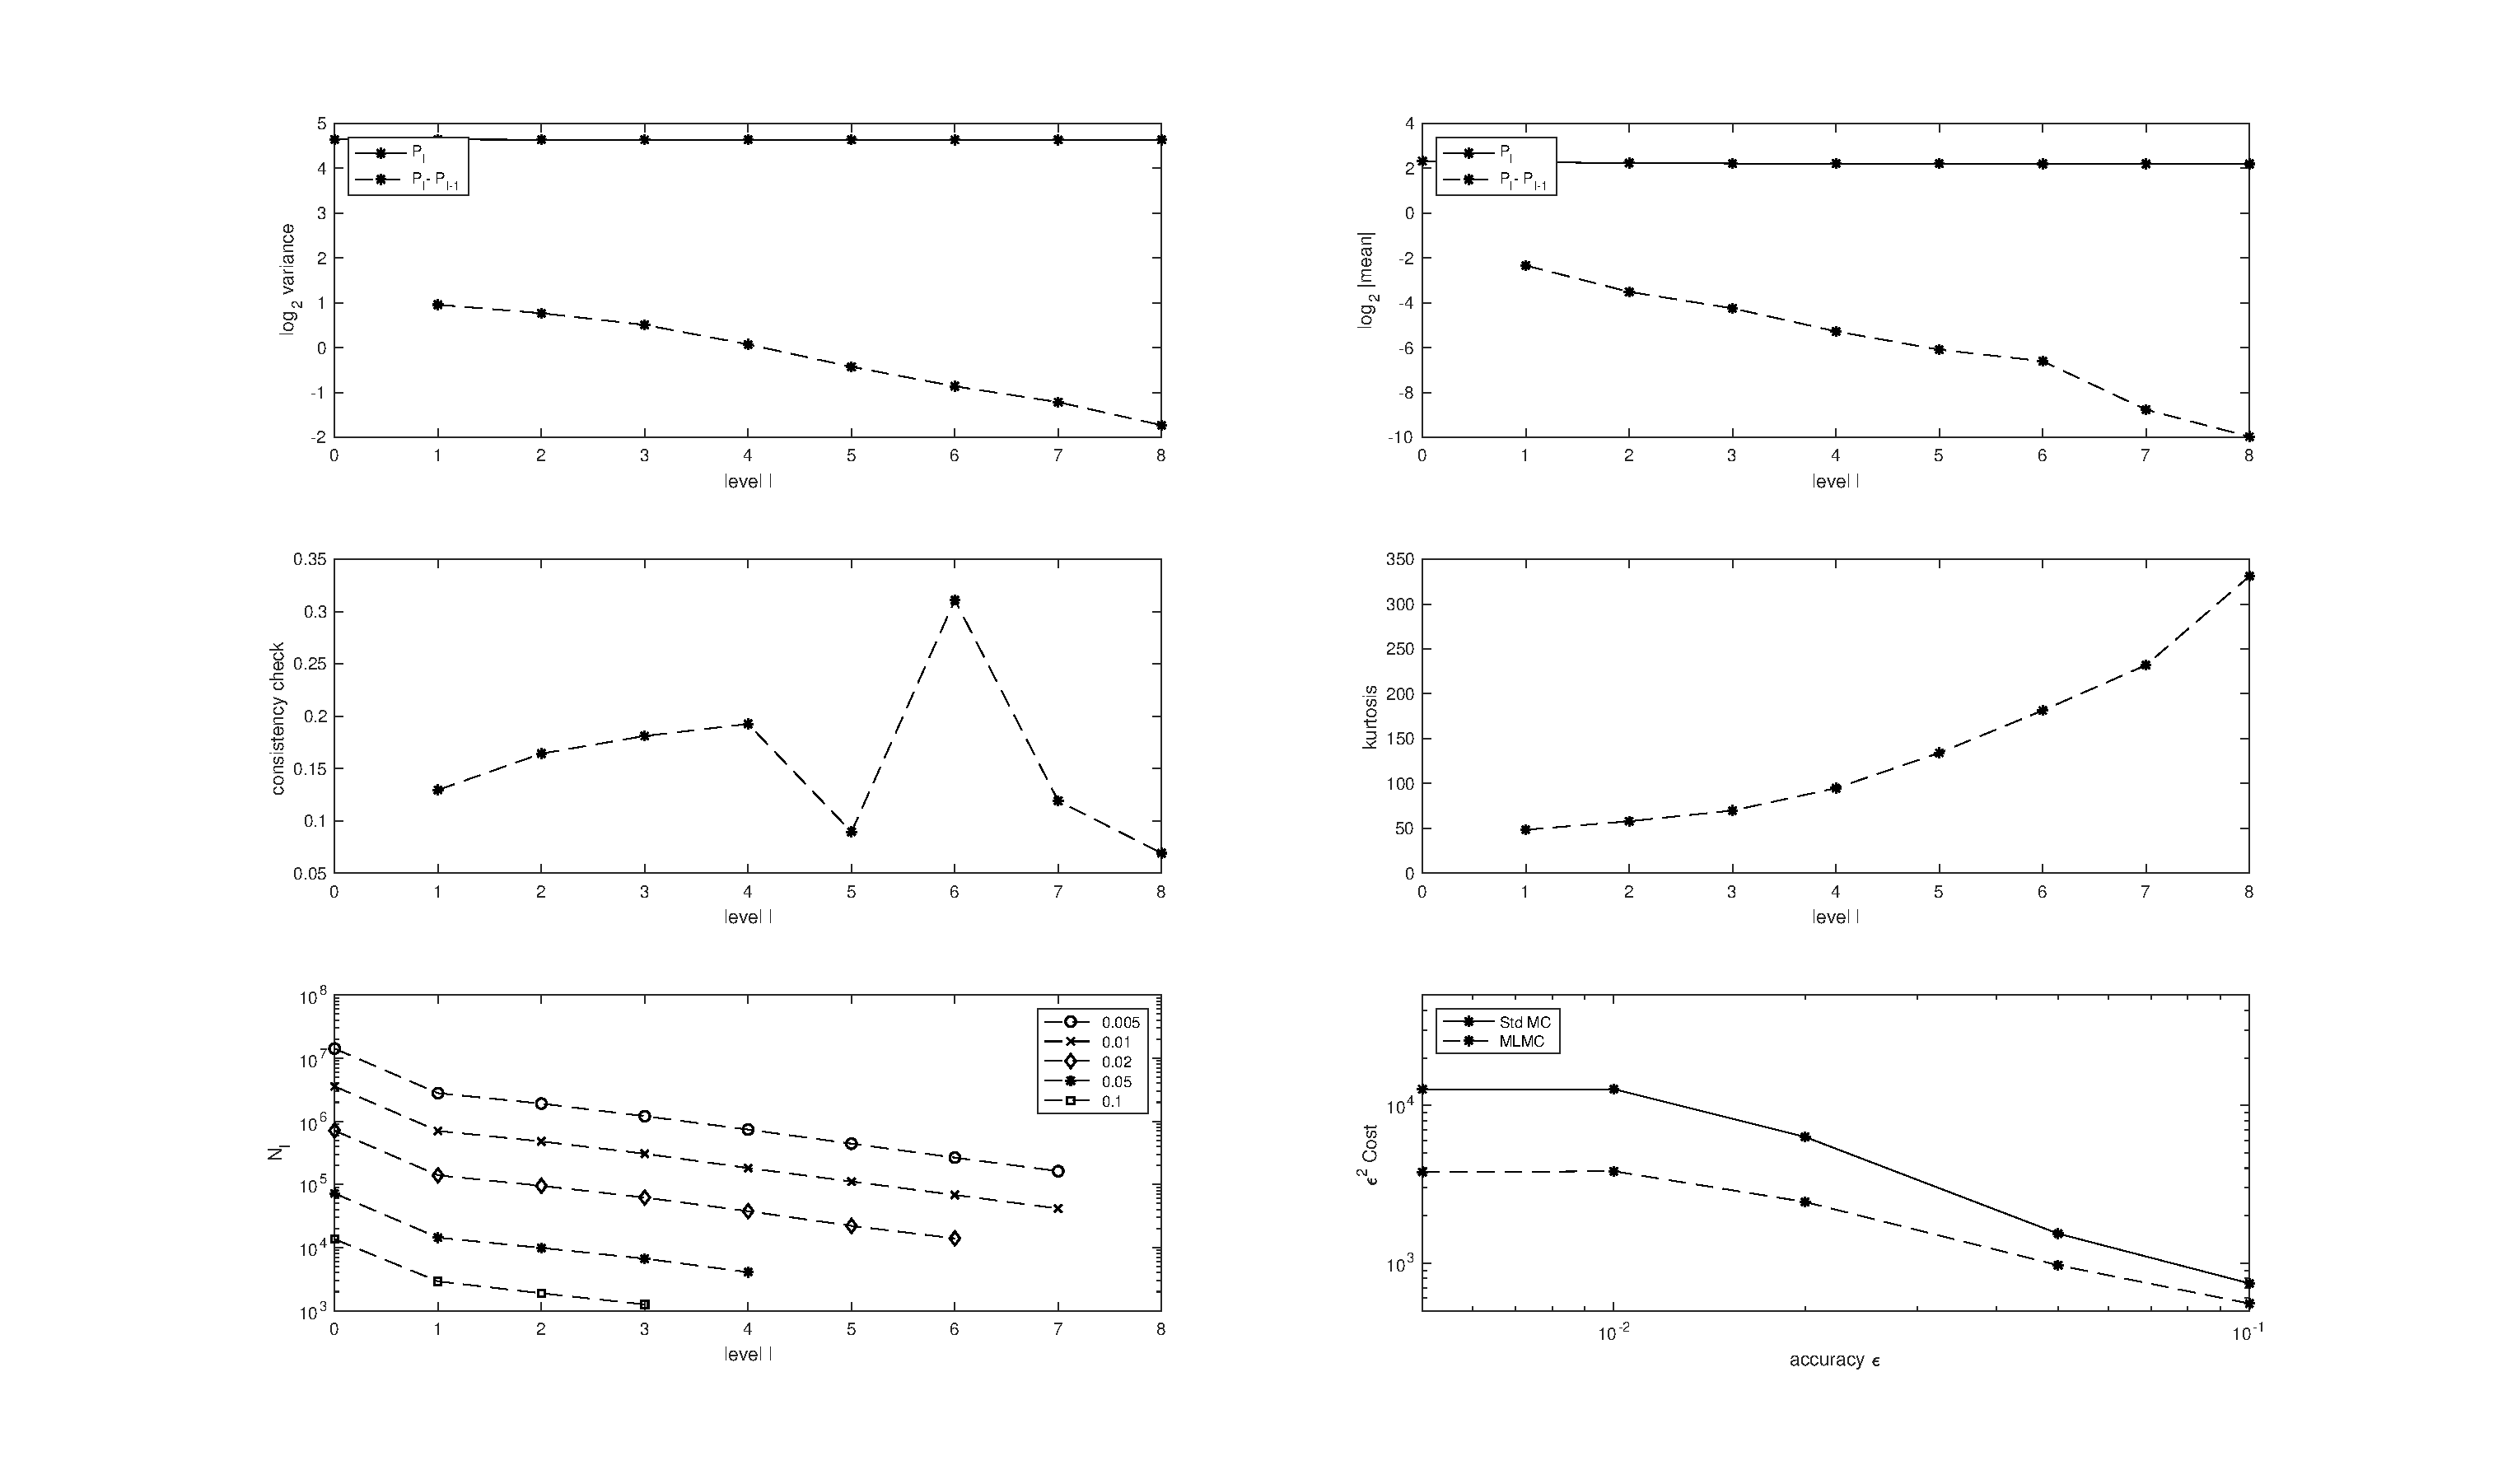
\includegraphics[width=1\linewidth]{./figures/MLMC_binary_opt/euler_digital_without_smoothing}

\caption{Numerical results for a digital call option using the MLMC method coupled with Euler-Maruyama discretisation of the GBM SDE, and without smoothing of the payoff.}
\label{fig:euler_digital_without_smoothing}
\end{figure}

\FloatBarrier

\FloatBarrier
	\begin{figure}[h!]
\centering
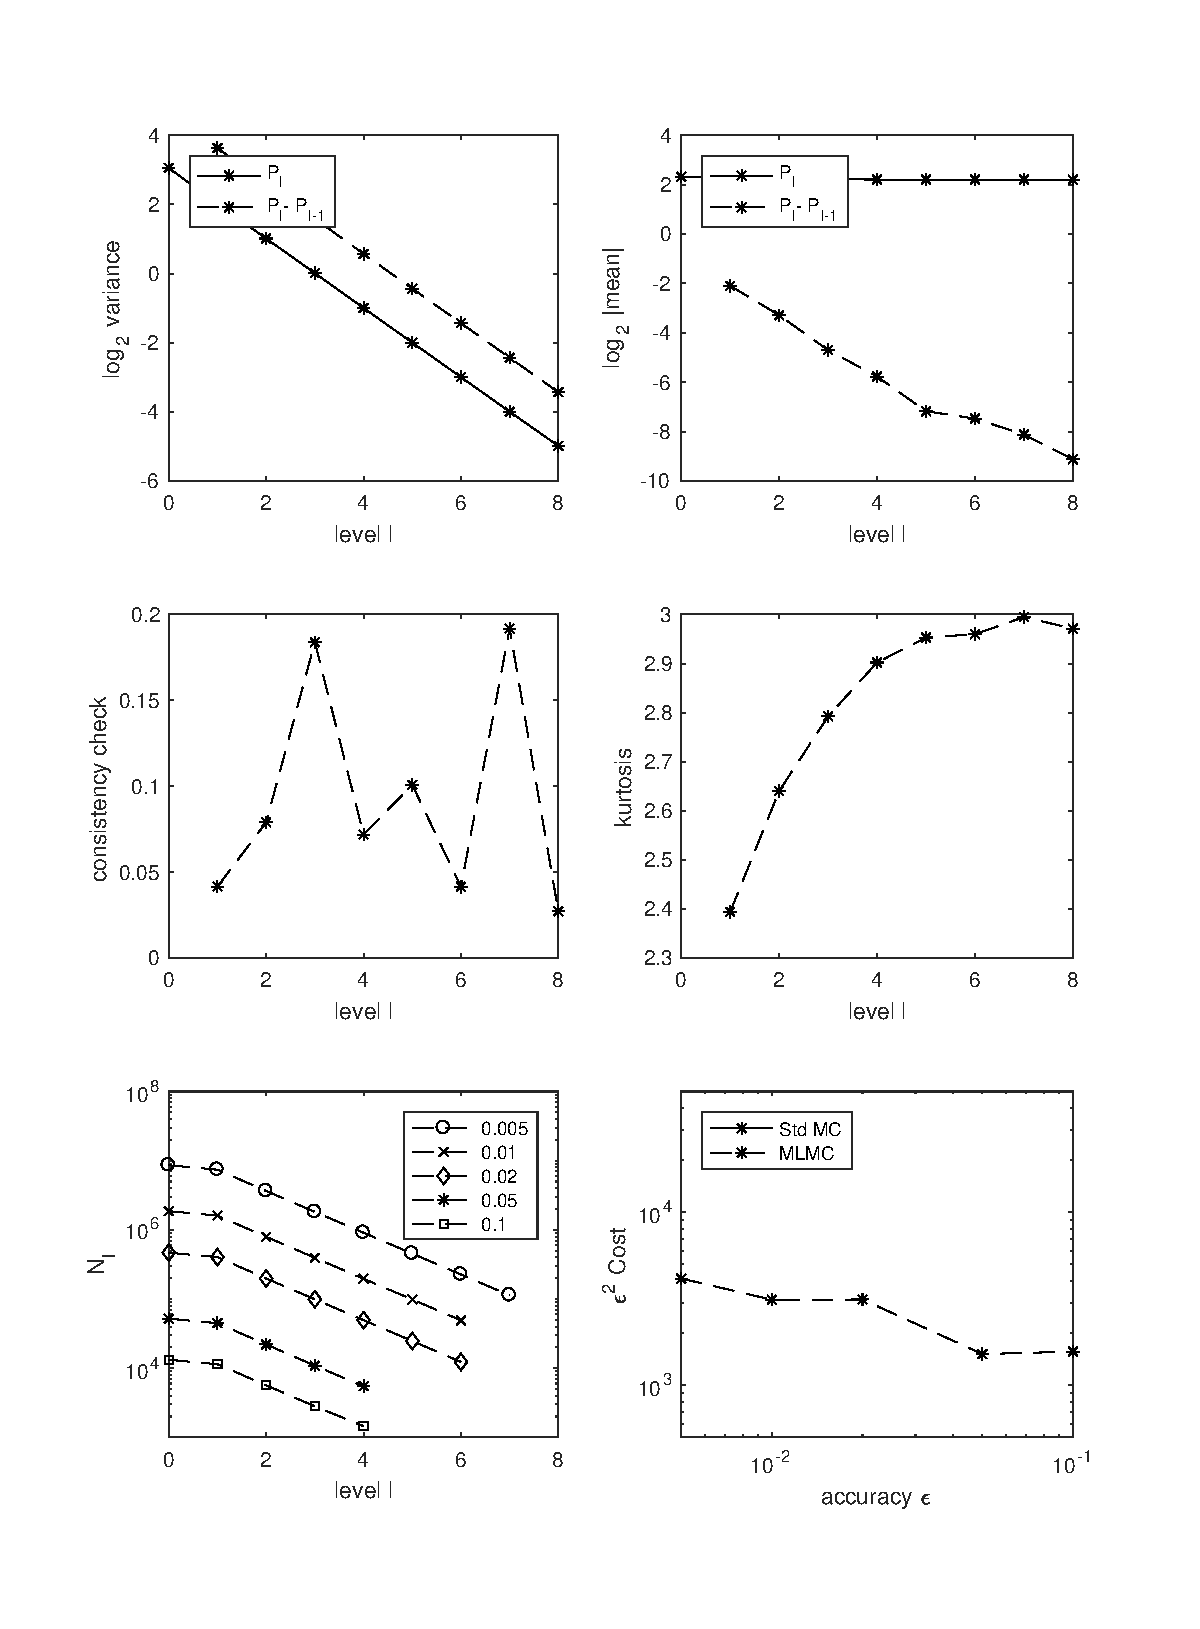
\includegraphics[width=0.7\linewidth]{./figures/MLMC_binary_opt/digital_option_with_smoothing_L_0_2_steps}

\caption{Numerical results for a digital call option using the MLMC method coupled with Euler-Maruyama discretisation of the GBM SDE, after applying  the numerical smoothing to the payoff.}
\label{fig:euler_digital_with_smoothing}
\end{figure}

\FloatBarrier


\subsection{MLMC for approximating densities and Greeks}\label{sec: MLMC for approximating densities and greeks}

